\documentclass[11pt,a4paper]{article}

\usepackage[utf8]{inputenc}
\usepackage[T1]{fontenc}
\usepackage[english]{babel}
\usepackage{amsmath,amssymb}
\usepackage{siunitx}
\usepackage{booktabs}
\usepackage{graphicx}
\usepackage{float}
\usepackage{geometry}
\usepackage{hyperref}

\geometry{margin=2.5cm}
\sisetup{
  per-mode=symbol,
  detect-all
}

\title{TP2 -- Switched-Capacitor Circuits}
\author{Léon \and Eliott}
\date{}

\begin{document}

\maketitle

\section{Objective}

The objective of this lab is to study switched-capacitor circuits and to use them to build a sinusoidal oscillator. First, a non-inverting switched-capacitor integrator is analyzed and simulated. Then two discrete-time oscillator structures are compared. Finally, a stable oscillator is simulated in order to generate a sinusoidal signal with a frequency in the range from \SI{2}{Hz} to \SI{20}{Hz}.

The sampling frequency is fixed at:
\[
f_e=\frac{1}{T_e}=\SI{1.0}{kHz},
\qquad
T_e=\SI{1}{ms}.
\]

\section{Non-Inverting Switched-Capacitor Integrator}

\subsection{Transfer Function}

The switched-capacitor integrator is defined by the capacitor ratio:
\[
k=\frac{C_1}{C_2}.
\]

At the end of phase $\Phi_2$, the charge sampled during the previous phase is transferred to the feedback capacitor. The output therefore satisfies the recurrence relation:
\[
V_s[n]-V_s[n-1]=kV_e[n-1].
\]

Taking the $z$-transform:
\[
V_s(z)-z^{-1}V_s(z)=kz^{-1}V_e(z).
\]

Thus:
\[
V_s(z)(1-z^{-1})=kz^{-1}V_e(z),
\]
and the transfer function is:
\[
I(z)=\frac{V_s(z)}{V_e(z)}
=
\frac{kz^{-1}}{1-z^{-1}}.
\]

This is the transfer function of a discrete-time integrator with one sample delay.

\subsection{Output for a Constant Input}

For:
\[
V_e=\SI{1.0}{V},
\qquad
V_s[0]=0,
\qquad
k=1,
\]
the recurrence becomes:
\[
V_s[n]=V_s[n-1]+1.
\]

Therefore, the ideal output over ten periods is:
\[
\begin{array}{c|ccccccccccc}
n & 0 & 1 & 2 & 3 & 4 & 5 & 6 & 7 & 8 & 9 & 10\\
\hline
V_s[n]\,(\mathrm{V}) & 0 & 1 & 2 & 3 & 4 & 5 & 6 & 7 & 8 & 9 & 10
\end{array}
\]

In a real or simulated circuit powered by $\pm\SI{5}{V}$, the output cannot increase indefinitely and saturates near the positive supply rail.

\subsection{LTspice Simulation}

The integrator was simulated with:
\[
C_1=C_2=\SI{10}{pF},
\qquad
k=1,
\qquad
V_e=\SI{1}{V}.
\]

The clock signals were:
\[
\Phi_1=\mathrm{PULSE}(0,5,0,10\mu s,10\mu s,480\mu s,1ms),
\]
\[
\Phi_2=\mathrm{PULSE}(0,5,500\mu s,10\mu s,10\mu s,480\mu s,1ms).
\]

\begin{figure}[H]
\centering
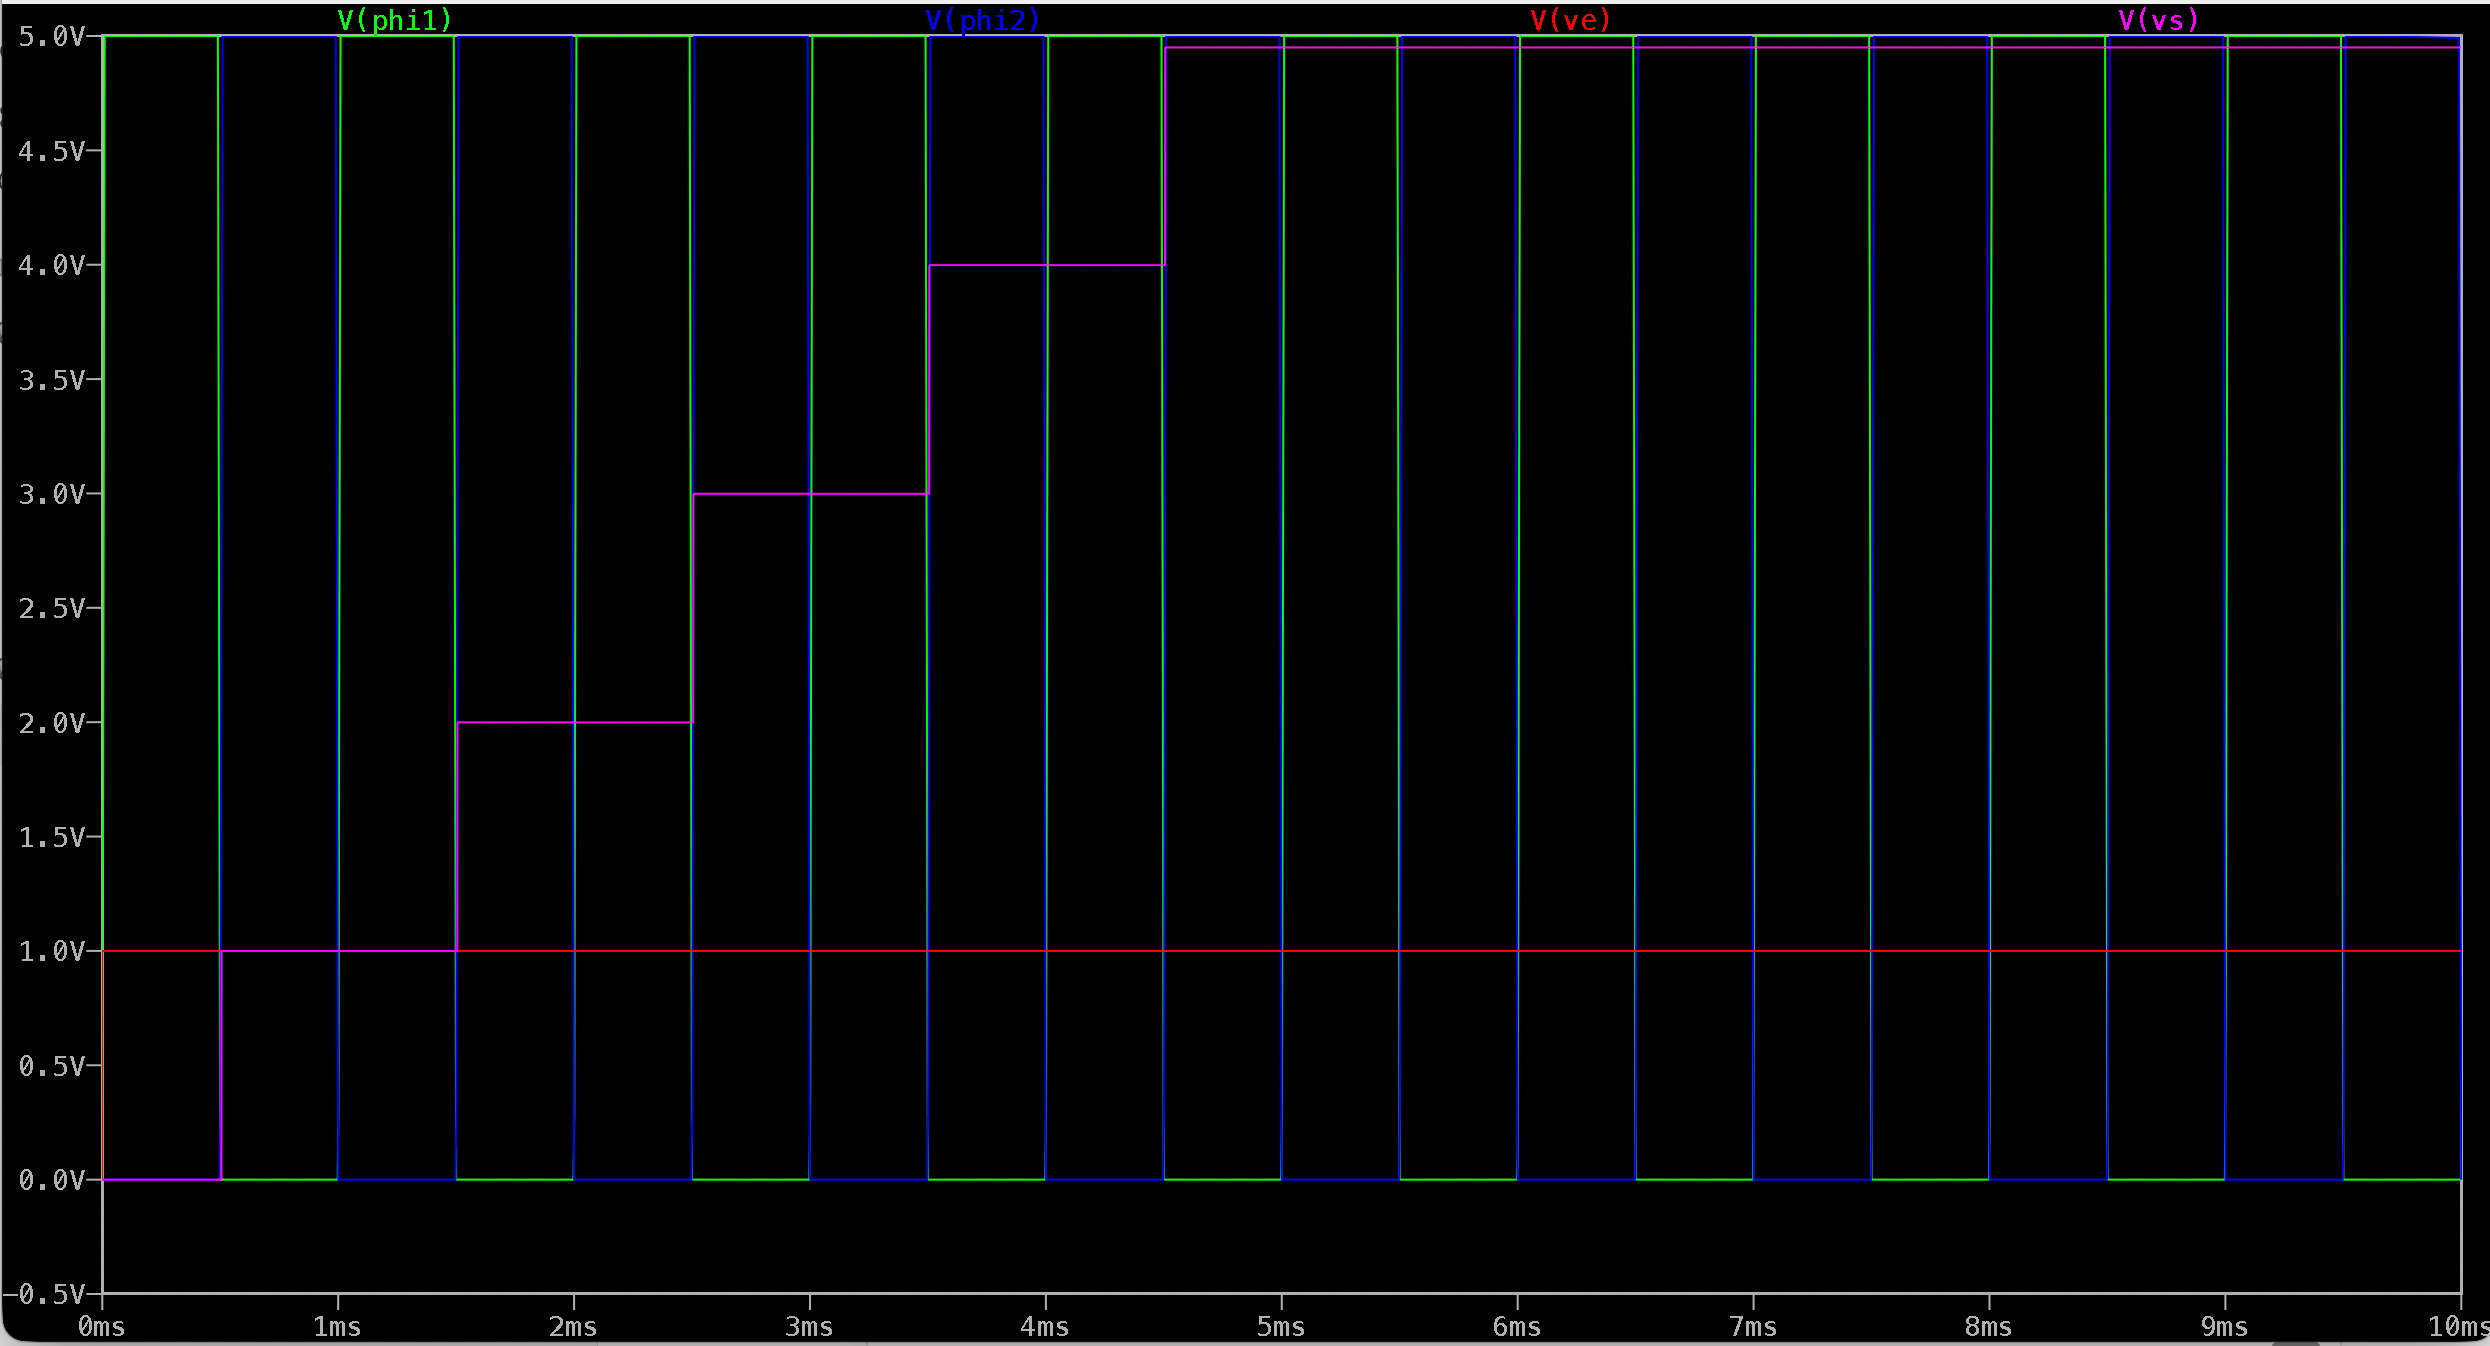
\includegraphics[width=0.95\textwidth]{Simulation1.png}
\caption{Simulation of the non-inverting switched-capacitor integrator.}
\end{figure}

The simulated output follows the expected staircase behavior at the beginning. Since $k=1$ and $V_e=\SI{1}{V}$, the output increases by approximately \SI{1}{V} per sampling period. After a few periods, the output saturates close to the positive supply voltage because the operational amplifier is powered by $\pm\SI{5}{V}$.

\section{First Oscillator}

\subsection{Discrete-Time Equations}

A sinusoidal signal satisfies:
\[
\frac{d^2x}{dt^2}+\omega_0^2x=0.
\]

This second-order equation can be written as two coupled first-order equations:
\[
\frac{dx}{dt}=\omega_0 y,
\qquad
\frac{dy}{dt}=-\omega_0 x.
\]

Using explicit Euler approximation:
\[
\frac{x[n+1]-x[n]}{T_e}=\omega_0 y[n],
\qquad
\frac{y[n+1]-y[n]}{T_e}=-\omega_0 x[n].
\]

Thus:
\[
x[n+1]=x[n]+k y[n],
\]
\[
y[n+1]=y[n]-k x[n],
\]
with:
\[
k=\omega_0T_e.
\]

These equations correspond to the original \texttt{gen-sin.m} script.

\subsection{Simulation Result}

The first oscillator was simulated with:
\[
k=0.05,
\qquad
N=1000,
\qquad
x[0]=1,
\qquad
y[0]=0.
\]

\begin{figure}[H]
\centering
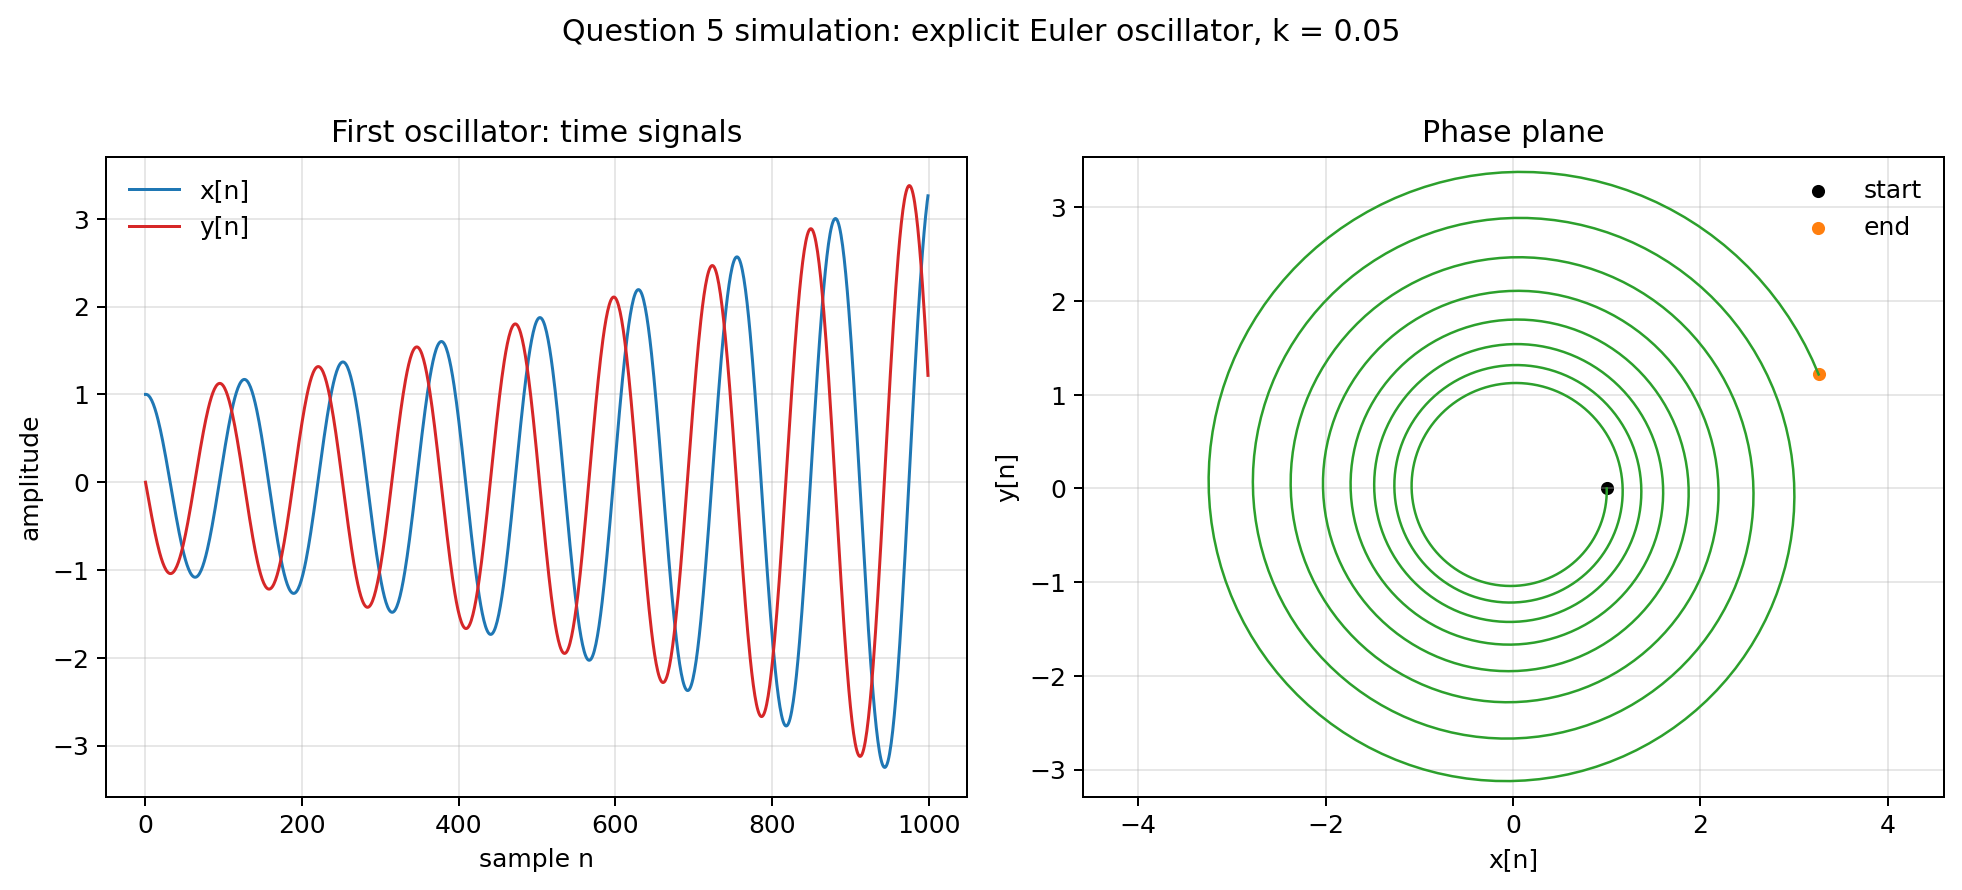
\includegraphics[width=0.95\textwidth]{Simulation2_Q5_first_oscillator_unstable.png}
\caption{Simulation of the first oscillator using explicit Euler equations.}
\end{figure}

The time-domain signals oscillate, but their amplitude increases with time. In the phase plane, the trajectory is an outward spiral rather than a closed curve. This shows qualitatively that the first oscillator is unstable.

\subsection{Stability Analysis}

The poles of the first oscillator are:
\[
z_{\pm}=1\pm jk.
\]

Their modulus is:
\[
|z_{\pm}|=\sqrt{1+k^2}.
\]

For any non-zero value of $k$:
\[
\sqrt{1+k^2}>1.
\]

Therefore, the poles are outside the unit circle and the system is unstable for $k>0$. This confirms the simulation result.

\section{Second Oscillator}

\subsection{Modified Equations}

To improve stability, the second integrator is modified so that the update of $y$ uses the new value of $x$. The equations become:
\[
x[n+1]=x[n]+k y[n],
\]
\[
y[n+1]=y[n]-k x[n+1].
\]

Equivalently:
\[
y[n+1]=y[n]-k(x[n]+ky[n]),
\]
so:
\[
y[n+1]=-kx[n]+(1-k^2)y[n].
\]

The state-space form is:
\[
\begin{bmatrix}
x[n+1]\\
y[n+1]
\end{bmatrix}
=
\begin{bmatrix}
1 & k\\
-k & 1-k^2
\end{bmatrix}
\begin{bmatrix}
x[n]\\
y[n]
\end{bmatrix}.
\]

\subsection{Simulation Result}

The script was modified by replacing the update loop with:
\[
x[i+1]=x[i]+k y[i],
\]
\[
y[i+1]=y[i]-k x[i+1].
\]

Using the same parameters as before:
\[
k=0.05,
\qquad
N=1000,
\qquad
x[0]=1,
\qquad
y[0]=0,
\]
we obtain the following result.

\begin{figure}[H]
\centering
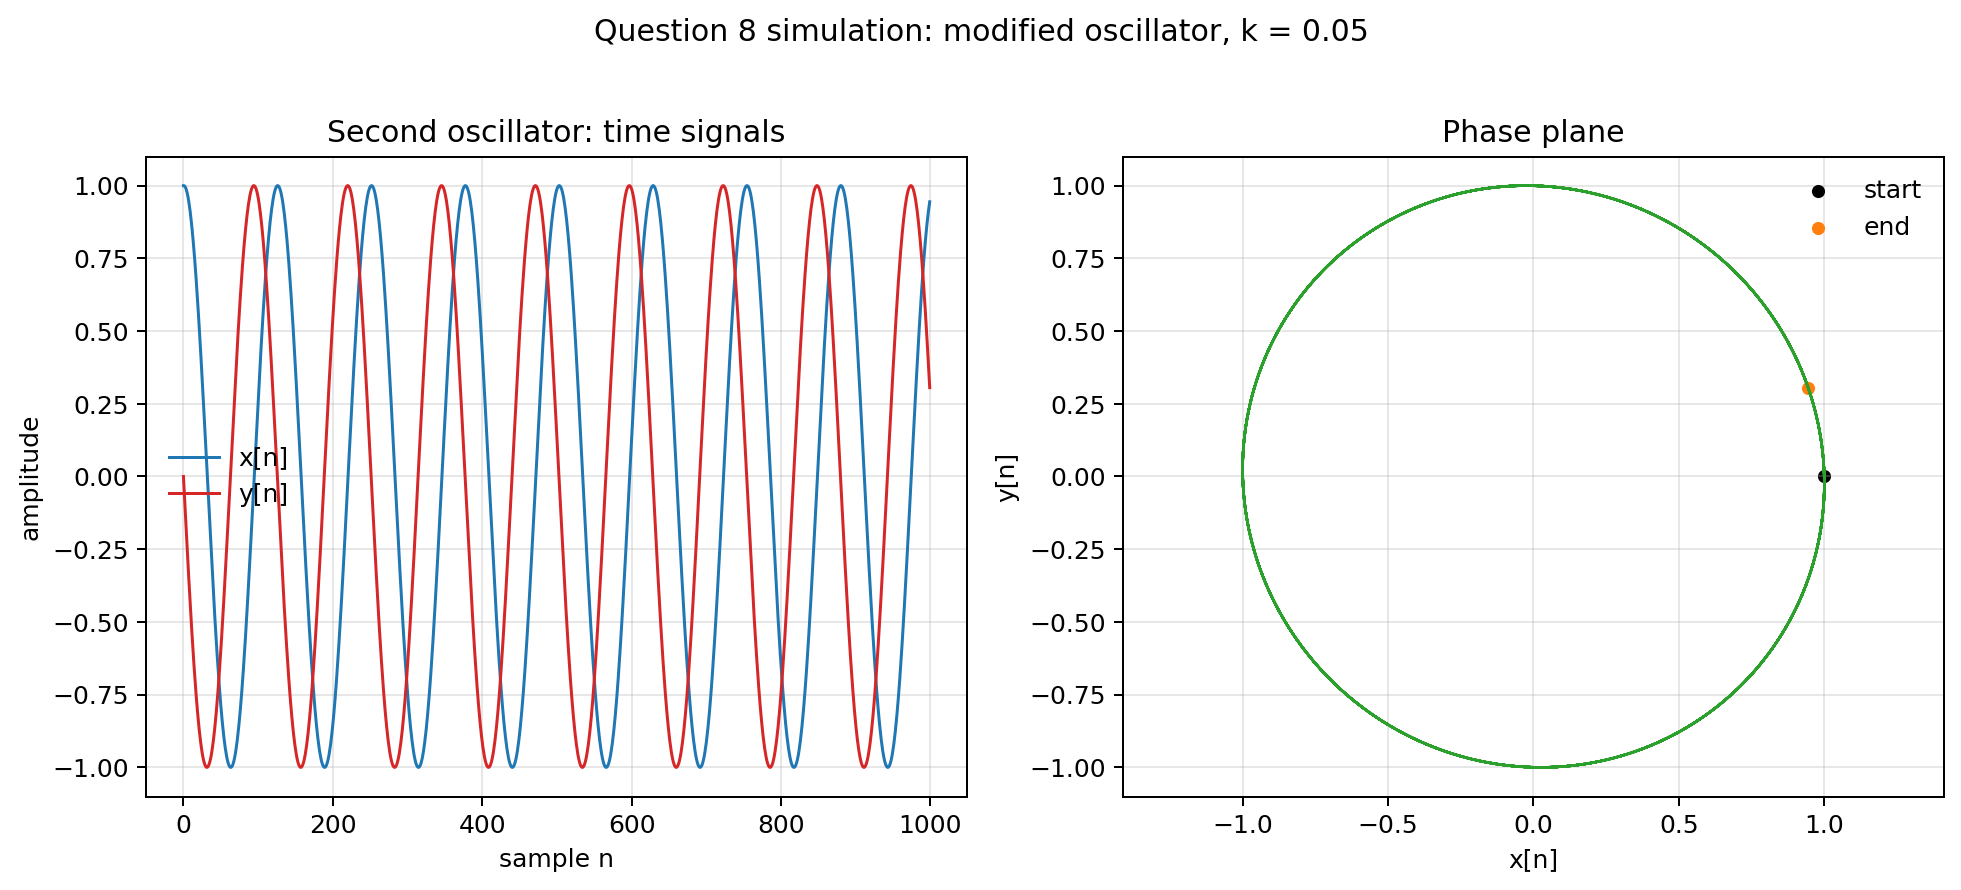
\includegraphics[width=0.95\textwidth]{Simulation2_Q8_second_oscillator_stable.png}
\caption{Simulation of the second oscillator with the modified update equation.}
\end{figure}

The signals remain bounded and the phase-plane trajectory is closed. This shows that the modified oscillator is stable or marginally stable for this value of $k$.

\subsection{Stability Condition}

For the second oscillator, the poles are given by:
\[
z_{\pm}
=
\frac{2-k^2\pm jk\sqrt{4-k^2}}{2},
\qquad k\leq 2.
\]

For $0<k<2$, the poles are complex conjugates. Their modulus is:
\[
|z_{\pm}|^2
=
\left(\frac{2-k^2}{2}\right)^2
+
\left(\frac{k\sqrt{4-k^2}}{2}\right)^2.
\]

Developing the numerator:
\[
|z_{\pm}|^2
=
\frac{(2-k^2)^2+k^2(4-k^2)}{4}
=
\frac{4}{4}
=1.
\]

Thus, for:
\[
\boxed{0<k<2},
\]
the poles lie on the unit circle and the oscillation remains bounded. For $k>2$, the poles become real and one of them has a modulus larger than 1, so the system becomes unstable.

\section{Sinusoidal Generator in LTspice}

\subsection{Choice of $k$ and $C_1$}

For the stable oscillator, the poles can be written as:
\[
z_{\pm}=e^{\pm j\theta}.
\]

From the real part:
\[
\cos\theta=1-\frac{k^2}{2}.
\]

Therefore:
\[
\theta=2\arcsin\left(\frac{k}{2}\right).
\]

The oscillation frequency is:
\[
f_0=\frac{\theta}{2\pi T_e}
=
\frac{f_e}{2\pi}\theta.
\]

Thus:
\[
k=2\sin\left(\pi\frac{f_0}{f_e}\right).
\]

With:
\[
f_e=\SI{1000}{Hz},
\qquad
C_2=\SI{10}{pF},
\]
we have:
\[
C_1=kC_2.
\]

For $f_0=\SI{2}{Hz}$:
\[
k=2\sin\left(\pi\frac{2}{1000}\right)
\approx 0.01257,
\]
\[
C_1\approx 0.01257\times\SI{10}{pF}
\approx \SI{0.126}{pF}.
\]

For $f_0=\SI{20}{Hz}$:
\[
k=2\sin\left(\pi\frac{20}{1000}\right)
\approx 0.1256,
\]
\[
C_1\approx 0.1256\times\SI{10}{pF}
\approx \SI{1.26}{pF}.
\]

\subsection{Startup of the Oscillator}

In an ideal simulation with zero initial conditions:
\[
x[0]=0,
\qquad
y[0]=0,
\]
the oscillator remains at rest:
\[
x[n]=0,
\qquad
y[n]=0.
\]

Therefore, a startup perturbation is required. In practice, this perturbation can come from noise, offset voltages, charge injection from the switches, or non-zero initial charge on the capacitors. In the simulation, a pulse is added to initiate the oscillation.

\begin{figure}[H]
\centering
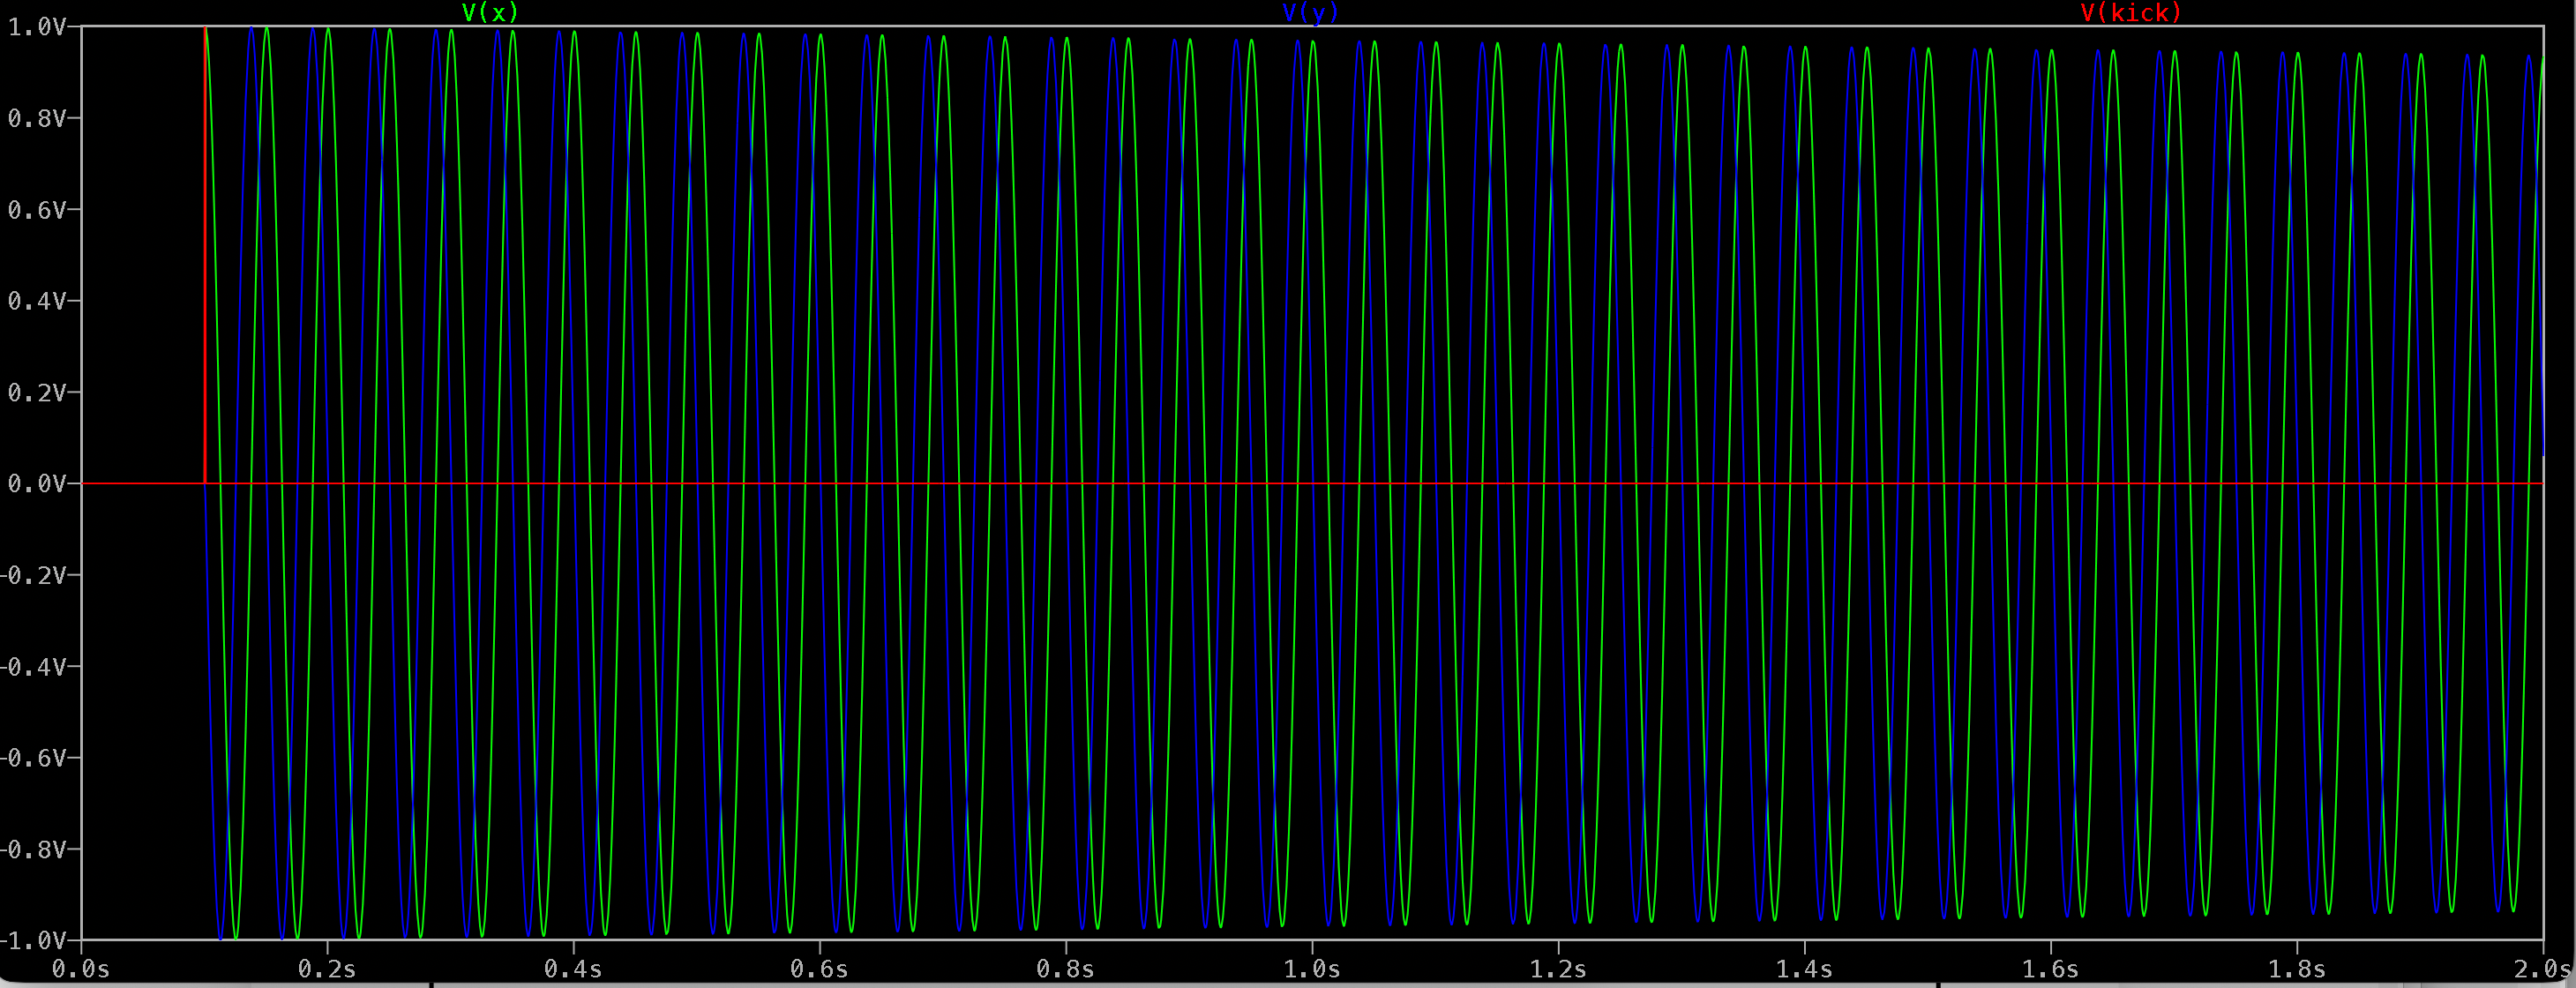
\includegraphics[width=0.95\textwidth]{simulation3.png}
\caption{Simulation 3: startup pulse and sustained oscillations of $x$ and $y$.}
\end{figure}

Before the startup pulse, both $x$ and $y$ remain equal to zero. After the pulse is applied, the oscillator starts. The two signals are phase-shifted and remain bounded, which confirms that the second oscillator structure can generate a stable sinusoidal signal.

\section{Influence of the Sampling Frequency}

The sampling frequency $f_e$ is fixed at the beginning of the lab, while the oscillation frequency is tuned by changing $k$, and therefore $C_1$.

Increasing $f_e$ improves the quality of the generated signal. For the same oscillation frequency, there are more samples per period, the waveform is closer to a continuous sinusoid, and the discretization error is reduced. However, a higher sampling frequency requires faster switches and a faster operational amplifier. It can also increase power consumption and make clock feedthrough or charge injection more critical. Moreover, for a fixed $f_0$, increasing $f_e$ reduces:
\[
k=2\sin\left(\pi\frac{f_0}{f_e}\right),
\]
so $C_1$ becomes smaller and harder to implement accurately.

Decreasing $f_e$ has the opposite effect. The circuit speed requirements are relaxed and $C_1$ can be larger, but the waveform quality becomes worse because there are fewer samples per period. The discretization error increases, and the signal may contain more sampling artifacts. The oscillation frequency must also remain well below the Nyquist frequency $f_e/2$.

\section{Summary}

\begin{table}[H]
\centering
\begin{tabular}{lll}
\toprule
Quantity & Value & Comment \\
\midrule
$f_e$ & \SI{1.0}{kHz} & Sampling frequency \\
$T_e$ & \SI{1}{ms} & Sampling period \\
$C_2$ & \SI{10}{pF} & Fixed capacitor \\
Integrator transfer function & $\dfrac{kz^{-1}}{1-z^{-1}}$ & Non-inverting integrator \\
First oscillator poles & $1\pm jk$ & Unstable for $k>0$ \\
Second oscillator stability & $0<k<2$ & Bounded oscillation \\
$k$ for \SI{2}{Hz} & $0.01257$ & $f_e=\SI{1}{kHz}$ \\
$C_1$ for \SI{2}{Hz} & \SI{0.126}{pF} & $C_1=kC_2$ \\
$k$ for \SI{20}{Hz} & $0.1256$ & $f_e=\SI{1}{kHz}$ \\
$C_1$ for \SI{20}{Hz} & \SI{1.26}{pF} & $C_1=kC_2$ \\
\bottomrule
\end{tabular}
\caption{Summary of the main theoretical and simulation results.}
\end{table}

\section{Conclusion}

This lab demonstrated how switched-capacitor circuits can implement discrete-time integrators and oscillators. The non-inverting switched-capacitor integrator behaves as expected: for a constant input and $k=1$, its output increases by approximately \SI{1}{V} at each sampling period until saturation occurs.

The first oscillator, based on two explicit Euler updates, is unstable because its poles are located outside the unit circle. This behavior was confirmed by the simulation, where the phase trajectory spirals outward. The second oscillator modifies the update equation and has poles on the unit circle for $0<k<2$, leading to bounded oscillations.

For a target frequency of \SI{20}{Hz} with $f_e=\SI{1}{kHz}$ and $C_2=\SI{10}{pF}$, the required capacitor value is $C_1\approx\SI{1.26}{pF}$. The LTspice simulation also shows that a startup pulse is necessary when the ideal initial conditions are zero. After this perturbation, the oscillator generates stable sinusoidal signals.

\end{document}
